
\chapter{The Framework Frontend}\label{frontend}

    In this chapter, the frontend of the presented framework is explained. It presents a graphical modeling tool where the user can model a desired car E/E architecture or vehicle topology comprising various hardware/software components. In the following, the details of the framework's frontend are described.
    
    %In addition, the inputs and outputs introduced in figure~\ref{approach} are illustrated in the front end.   



    
    \section{Modeling} 
    
    Modeling is a powerful and versatile technique used across various fields to represent, simulate, or describe real-world systems, processes, or phenomena. It involves creating simplified, abstract representations of complex entities to gain insights, make predictions, or solve problems. Modeling aims to capture the essential features and behaviors of the subject being studied while discarding unnecessary details. In today's fast-paced automotive industry, where innovation drives, creating cutting-edge vehicles requires a seamless integration of complex electrical and electronic systems. This is where sophisticated modeling tools step in, empowering automotive engineers to bring their ideas to life with precision and efficiency. 
    
    The proposed framework includes a frontend providing the modeling functionality. 
    The user can graphically design E/E architectures and car topologies using the introduced tool. Figure~\ref{fig5} presents a designed example utilizing our tool where, after creating a project, the user is able to select various hardware/software components such as a gateway, network switch, application, ECU, HPCU, communication message, communication task, etc~\cite{askaripoor2023designer}. 
    %In the context of engineering, science, and technology, modeling serves as an indispensable tool for understanding, designing, and optimizing systems. It enables researchers, engineers, and analysts to work with a virtual representation of their subject, allowing them to experiment, validate hypotheses, and study the effects of different variables without the need for costly and time-consuming real-world experiments.
   

    \subsection{Web-based Modeling Tool}
    
    The E/E Designer framework uses a web-based frontend. In the following, several advantages of web-based tools are illustrated.
    
    One of the key advantages of web-based modeling tools is their accessibility. They can be accessed from any device with an internet connection, eliminating the need for specific software installations~\cite{askaripoor2023designer}. This accessibility allows for collaboration and sharing of models across different teams, locations, and devices. In addition, it eases collaboration among team members. Multiple users can work on the same model simultaneously, making collaborating, discussing, and making real-time updates easier. This enhances team productivity and reduces the time spent on model synchronization and version control. Also, changes made by one user are instantly visible to all other users. This enables real-time updates and fosters efficient communication and decision-making within the team. It eliminates the need for manual merging of changes and reduces the chances of errors or conflicts in the model.
    Web-based modeling tools can quickly scale to accommodate projects of varying sizes and complexities. They can handle large models with extensive diagrams, multiple components, and interconnected systems. The cloud-based infrastructure of these tools enables seamless scaling without the need for additional hardware or software upgrades.
    \begin{figure}[t]
    	\centering
    	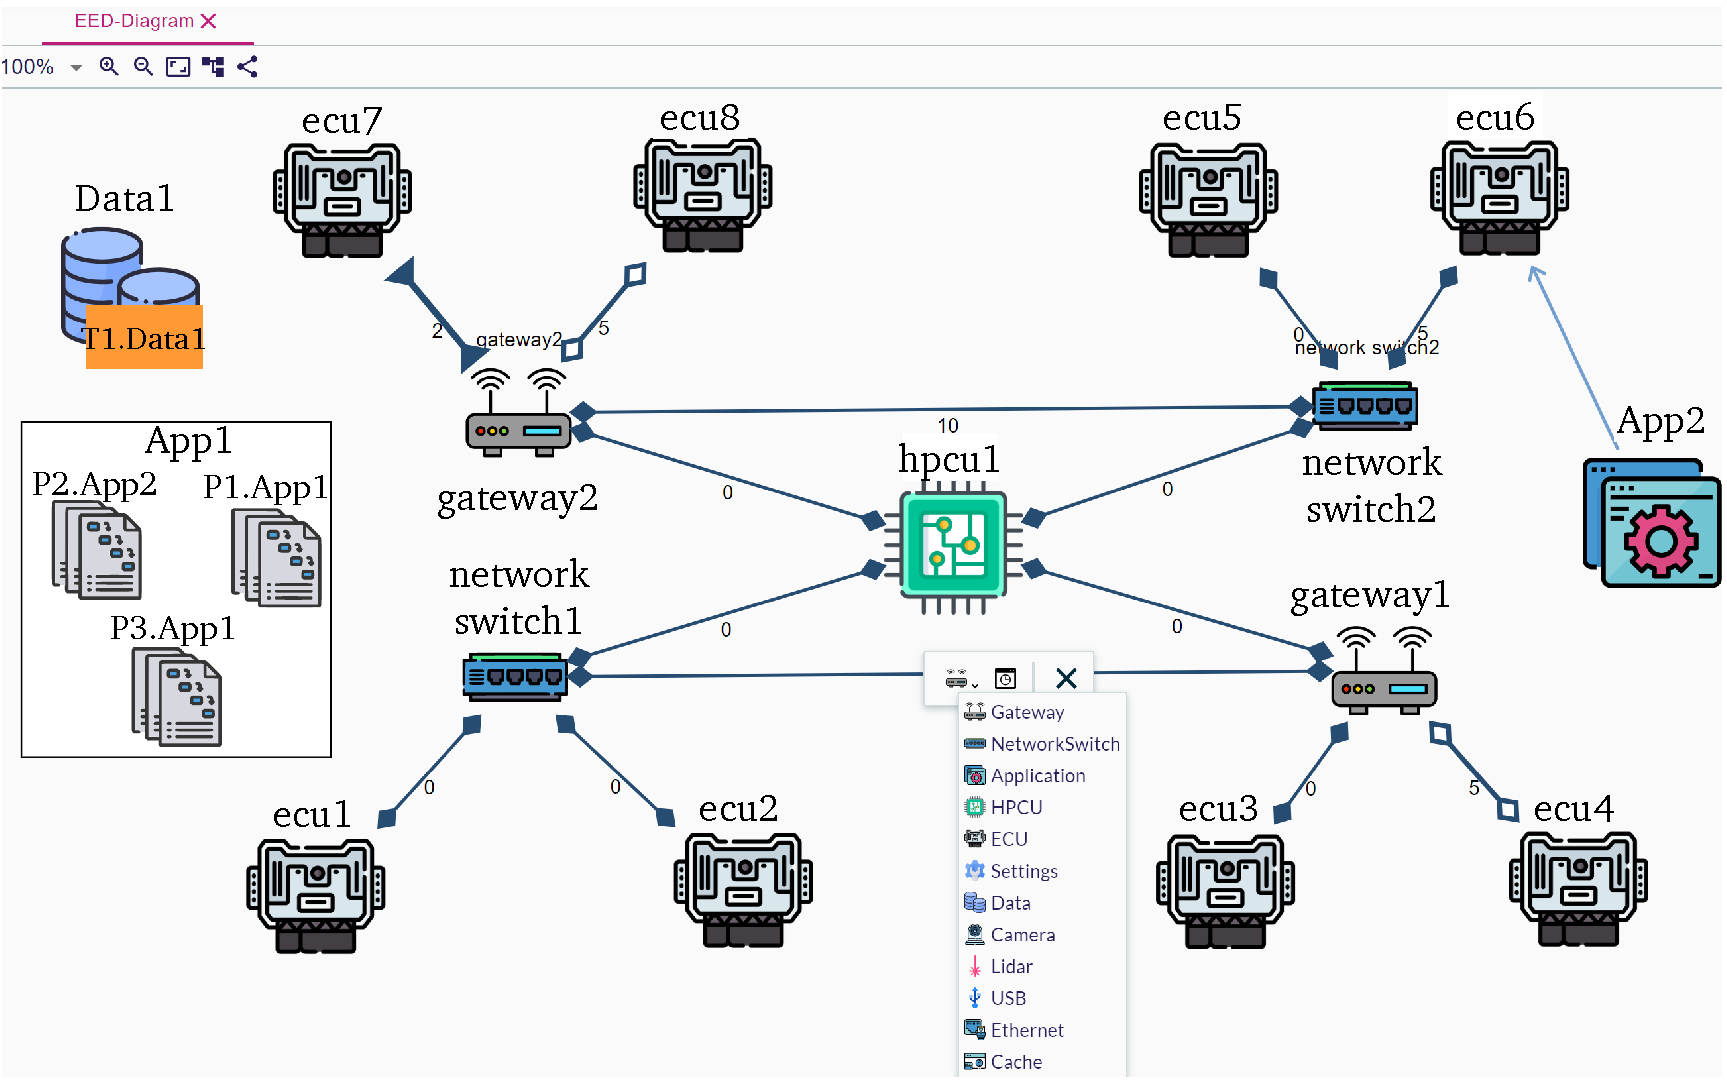
\includegraphics[width=1\textwidth]{figures/ee_model1.pdf}
    	\caption{ An example of zonal E/E architecture model using the presented model-based framework~\cite{askaripoor2023designer}.}
    	\label{fig5}
    \end{figure}
    They often come with built-in version control features. This allows users to track and manage different versions of the model, view revision history, and revert to previous versions if needed. Version control ensures the model remains consistent and provides a safety net for experimentation and exploration.
    
     The web-based frontend stores models and associated data in a centralized location like a cloud server. This centralized storage ensures that the latest version of the model is always accessible and eliminates the risk of data loss due to hardware failures or local storage issues. It also provides a secure backup and facilitates easy sharing and retrieval of models. Another feature of the web-based tools is cross-platform compatibility. This makes them compatible with different operating systems and platforms. Users can access and use these tools on Windows, Mac, Linux, or any other platform that supports a modern web browser. This feature enhances flexibility and convenience for users.
     Another advantage of web-based tools is integration capabilities with other software tools and systems. They can be easily integrated with version control systems, requirements management tools, issue trackers, and various development environments. Additionally, web-based tools often provide application programming interfaces (APIs) and extensibility options, allowing users to customize and extend the functionality of the tool to suit their specific needs.
     
    The E/E Designer consists of a web-based frontend where all above-explained features are supported.      
    %Cross-Platform Compatibility: Web-based modeling tools are typically built using web technologies, making them compatible with different operating systems and platforms. Users can access and use these tools on Windows, Mac, Linux, or any other platform that supports a modern web browser. This cross-platform compatibility enhances flexibility and convenience for users.
    
    %In summary, web-based modeling tools offer enhanced accessibility, collaboration, real-time updates, version control, scalability, centralized data storage, integration capabilities, and cross-platform compatibility. These advantages make them a popular choice for modeling and design tasks, enabling efficient and effective collaboration among team members and supporting the evolving needs of modern software and system development.


     
     
     
     %and the \textit{E/E Designer}'s outputs into the \textit{Sirius Web} project, both its frontend and backend were modified and developed.

 
 
     \subsection{Drag and Drop Functionality}
     
    The E/E Designer tool supports drag-and-drop functionality, a valuable feature in a modeler tool, as it provides an intuitive and user-friendly way to create and manipulate models. Here are some advantages of incorporating drag-and-drop functionality~\cite{askaripoor2023designer}.
    This feature simplifies the modeling process by allowing users to visually create and arrange elements in the model. Users can drag elements from a palette or toolbox and drop them onto the canvas, eliminating the need for manual drawing or coding. This intuitive approach makes the tool accessible to users with varying technical expertise. Moreover, users can quickly create models by selecting and placing predefined elements onto the canvas. This accelerates the E/E system development process and reduces the time required for the manual creation and positioning of model components. System integrators can focus more on the overall structure and logic of the E/E model rather than spending time on tedious placement and alignment tasks.
    Model elements can be easily modified and rearranged. Architects can drag existing elements to different locations on the canvas, change their connections, or even drag new elements into existing ones to create hierarchical relationships.
    
    %Improved Productivity: Drag and drop functionality streamlines the model creation process, leading to improved productivity. Users can quickly assemble models by dragging and dropping elements, allowing them to focus more on the actual design and logic of the model rather than manual placement tasks. This increased productivity enables faster iteration cycles and facilitates the development of complex models within shorter timeframes.
    %Enhanced Collaboration: Drag and drop functionality promotes collaboration among team members working on the same model. Users can easily share their models with others and collaborate by dragging and dropping elements into the shared model. This real-time collaboration improves communication, encourages knowledge sharing, and enables teams to work together seamlessly, regardless of their geographical locations.
    %Consistency and Standardization: Drag and drop functionality can be accompanied by predefined templates or design patterns. This promotes consistency and standardization in model creation, as users can drag and drop elements that adhere to predefined conventions or best practices. It ensures that models follow a consistent structure and layout, enhancing readability and maintainability.
     Based on the Figure~\ref{fig5}, after creating a project, users can select various hardware/software components, such as gateways, network switches, applications (including threads), ECUs (comprising sub-components like processors and memory), HPCUs (including sub-components such as processors, cores, memory, and GPUs), communication messages (in this case, data), communication tasks, and more. Clicking on an empty field brings up a window that displays the available objects that can be selected and generated. Furthermore, users can force applications to be mapped to specific hardware components before the solving step. For example, in Figure~\ref{fig5}, \textit{App$_2$} is forced to run on \textit{ECU$_6$} (blue arrow)~\cite{askaripoor2023designer}.
      %As can be observed in figure~\ref{fig5}, a window pops up after clicking on an empty field which particularly displays the HW/SW components that can be chosen and created. Furthermore, the applications can be forced to be mapped on a specific HW component before the solving step. For example, \textit{App$_2$} is forced to be run on \textit{ECU$_6$} (blue arrow) regarding figure~\ref{fig5}. 
    \begin{figure}[b!]
	\centering
	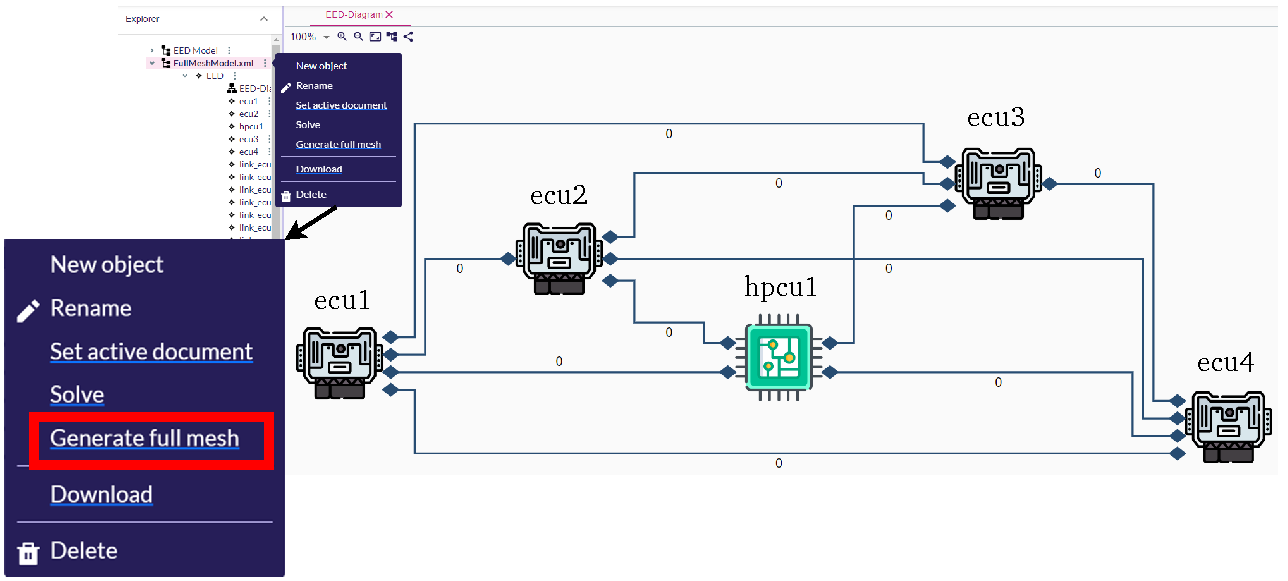
\includegraphics[width=1\columnwidth]{figures/fullmesh_option.pdf}
	\caption{A designed full-mesh E/E model including links and ECUs using the E/E Designer tool. By clicking on "Generate full-mesh", each hardware node is connected to other nodes.}
	\label{fig0007} 
    \end{figure}
    
    \subsection{Full-mesh Topology}
    In the context of E/E architecture, a full-mesh topology refers to a network configuration where every node (or component) is directly connected to every other node in the system. Each node serves as a point-to-point link with all other nodes, forming an extensive and redundant interconnection pattern.
    The full mesh topology is known for its robustness and fault tolerance because if one node fails, the communication pathways remain intact through alternative routes. However, this topology can become complex and costly as the number of nodes increases, as the number of connections grows exponentially~\cite{9565115,9212001,askaripoor2023designer}. To increase the design diversity and facilitate the modeling process, the framework supports a full-mesh generation option that creates a full-mesh network topology for selected hardware nodes where each node is connected directly to all other nodes (see Figure~\ref{fig0007}).
    
    
    \subsection{Automatic Creation of Software/Hardware Components}
    
    As hardware/software components increase, the modeling and drag-and-drop action become complex and time-consuming. For instance, a designer wants to model an architecture including 100 ECUs and 200 applications. This process takes considerable time. Consequently, an option is integrated into the framework that allows the users to have multiple components at once without dragging and dropping. This saves a significant amount of time for modeling extended topologies/architectures.      
 
 
    \begin{figure}[ht]
 	\centering
 	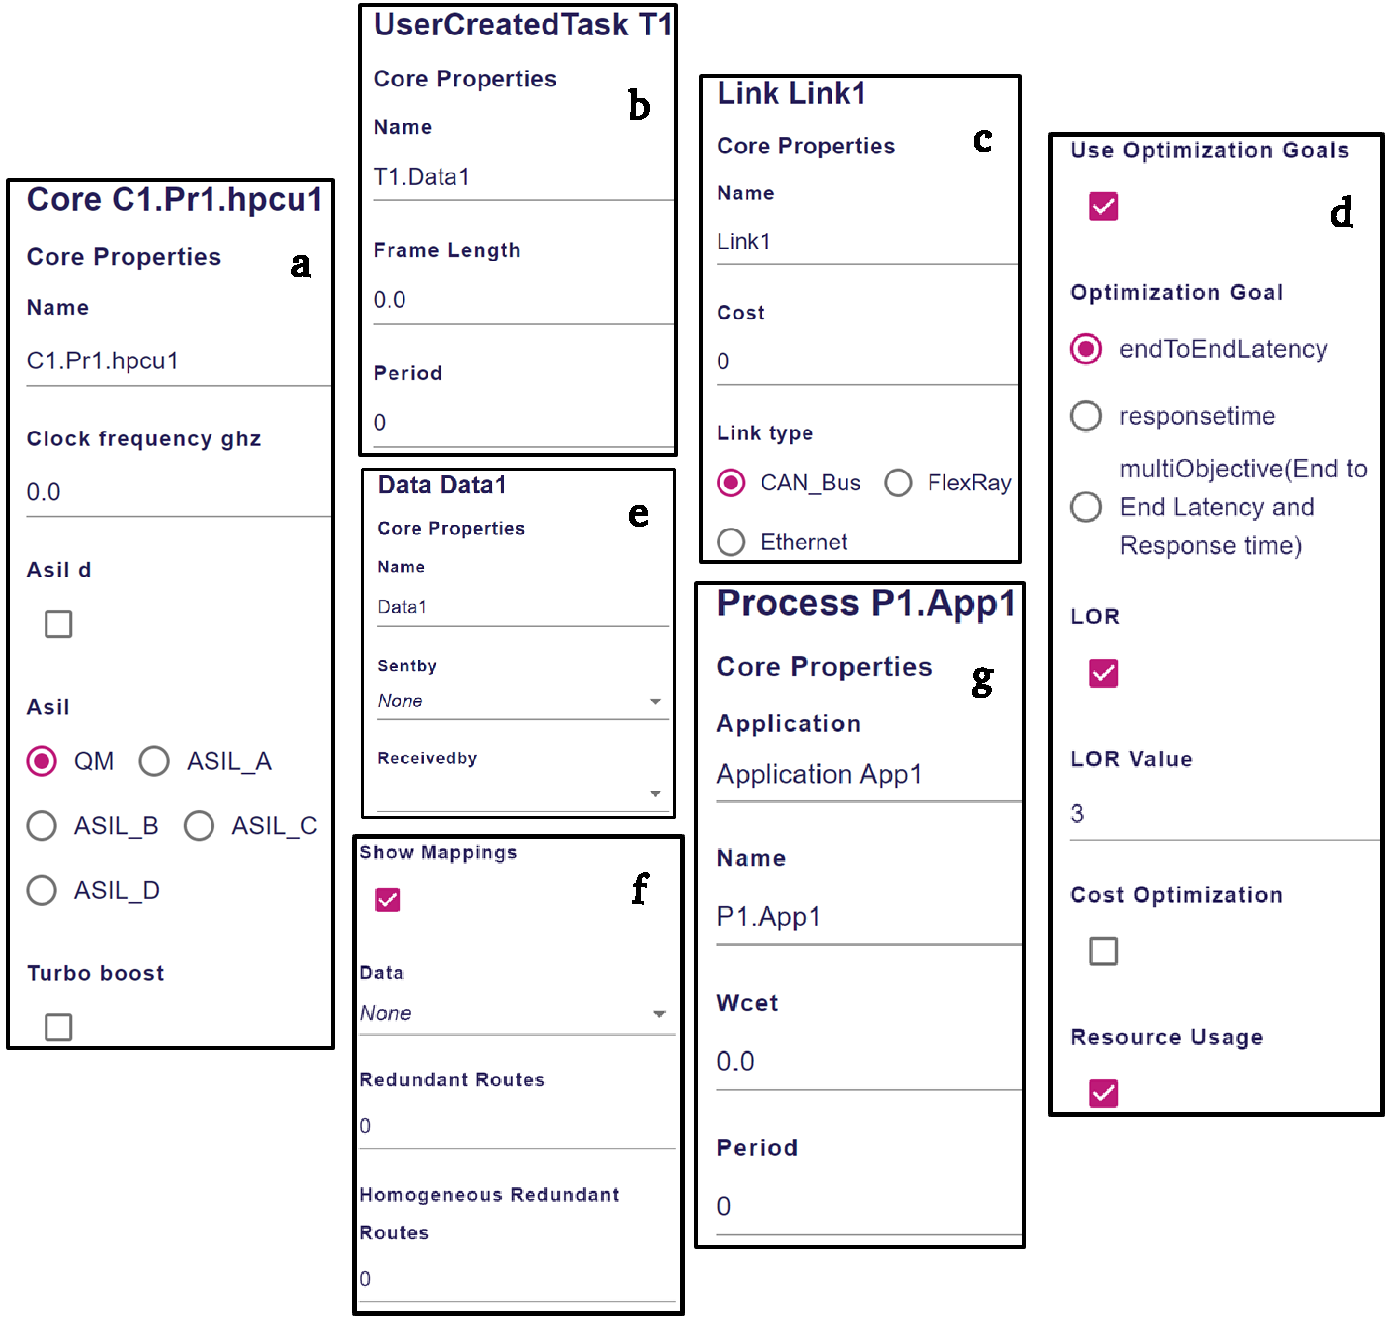
\includegraphics[width=1\textwidth]{figures/req1.pdf}
 	\caption{Component properties (a), (b), (c), (e), (g), and optimization and solving settings (d) and (f) in the frontend of the presented framework~\cite{askaripoor2023designer}.}
 	\label{fig6}
    \end{figure}
 
    \section{Requirements and Properties}
    In this section, all safety and non-safety requirements that can be chosen by the user in the frontend are discussed. Moreover, the properties regarding solving and optimization objectives integrated into the frontend are explained.
 
    \subsection{Hardware/Software Requirements and Properties}
 
 %Apart from modeling, each component's requirements and properties must be determined to solve a designed model. The details regarding several components and the solving settings are taken into consideration. For example, as part of an HPCU, a core can have various ASIL levels as a safety-critical property, a turbo boost feature, and an arbitrary name. While for a link's type (comprising Ethernet, FlexRay, and TT CAN bus), maximum bandwidth capacity, cost, and name can be selected. Moreover, each link type has a unique visualization symbol. For instance, \textit{ECU$_7$} and \textit{ECU$_8$} are connected with two different links to \textit{gateway$_2$} based on figure~\ref{fig5}. The application thread properties include the execution time, period, and name of each thread (in the tool named process). Moreover, an application can be defined as safety or non-safety-critical in the application properties and have a specified memory usage. Additionally, each communication task includes a name, frame length, and period as its properties. Also, the sender and receiver of a communication message can be specified.
 
 
    Apart from modeling, the requirements and properties relevant to each component can be determined, and they are a must-have for solving a designed model. The details of each component are displayed on the right side of the modeling window. Figure~\ref{fig6} illustrates the details regarding several components. As presented in Figure~\ref{fig6} (a), for example, as part of an HPCU, a core can have various ASIL levels as a safety-critical property, comprising ASILs A, B, C, D, and QM, a turbo boost feature, a defined clock frequency, a maximum memory utilization, a failure rate, interface to environment choice, and an arbitrary name. For a link, its type (comprising Ethernet, FlexRay, and TT CAN bus), maximum bandwidth capacity, cost, and name can be selected (refer to Figure~\ref{fig6} (c)). Moreover, each link's type has a unique visualization symbol, e.g., \textit{ECU$_7$} and \textit{ECU$_8$} are connected with two different links to \textit{gateway$_2$} based on Figure~\ref{fig5}. The application thread properties consist of the execution time, period, and name of each thread (in the tool named process), as shown in Figure~\ref{fig6} (g). It should be added that an application can be defined as safety or non-safety-critical in the application properties and have a determined memory usage. Also, the ASIL level of each application can be specified similarly to the core's properties. Additionally, each communication task includes a name, frame length, and period as its properties, as displayed in Figure~\ref{fig6} (b). Also, the sender and receiver of a communication message can be specified as Data details depicted in Figure~\ref{fig6}~(e)~\cite{askaripoor2023designer}. 
 
    \subsection{Optimization and Solving Properties}

 
    As mentioned in Chapter \ref{method}, the presented model-based framework supports several requirements, optimization goals, and multi-objective optimization~\cite{askaripoor2023designer, 9565115}. Hence, a setting module has been integrated into the frontend where the user can choose the multi-objective type, activate or deactivate the whole optimization method (\textit{Use Optimization Goals} checkbox in Figure~\ref{fig6} (d)), each objective and boundary constraint/requirement, e.g., LOR and LOR maximum tolerable bound, maximum bandwidth utilization, RU, maximum resource utilization, maximum reliability, and cost (see Figure~\ref{fig6} (d)). Furthermore, the type of route, such as single, multi-cast, redundant, homogeneous redundant, and the number of required homogeneous redundant paths, can be chosen as indicated in Figure~\ref{fig6}~(f). 
    
    %number of redundant and homogeneous redundant routes as the safety-critical requirements are able to be modified. In addition, to have a clear visualization of the solution in the front end, each created route and mapping only for a related message are shown. This can be selected by the user in the Data section presented in figure~\ref{fig6} (d).       
 
    \section{Solving and Solutions}
    
    After modeling a vehicle's topology and defining the requirements and properties related to the components, optimizations, and solving, the designed E/E architecture is ready to be solved and optimized. 
    
    
    
    
    \begin{figure}[t]
	\centering
	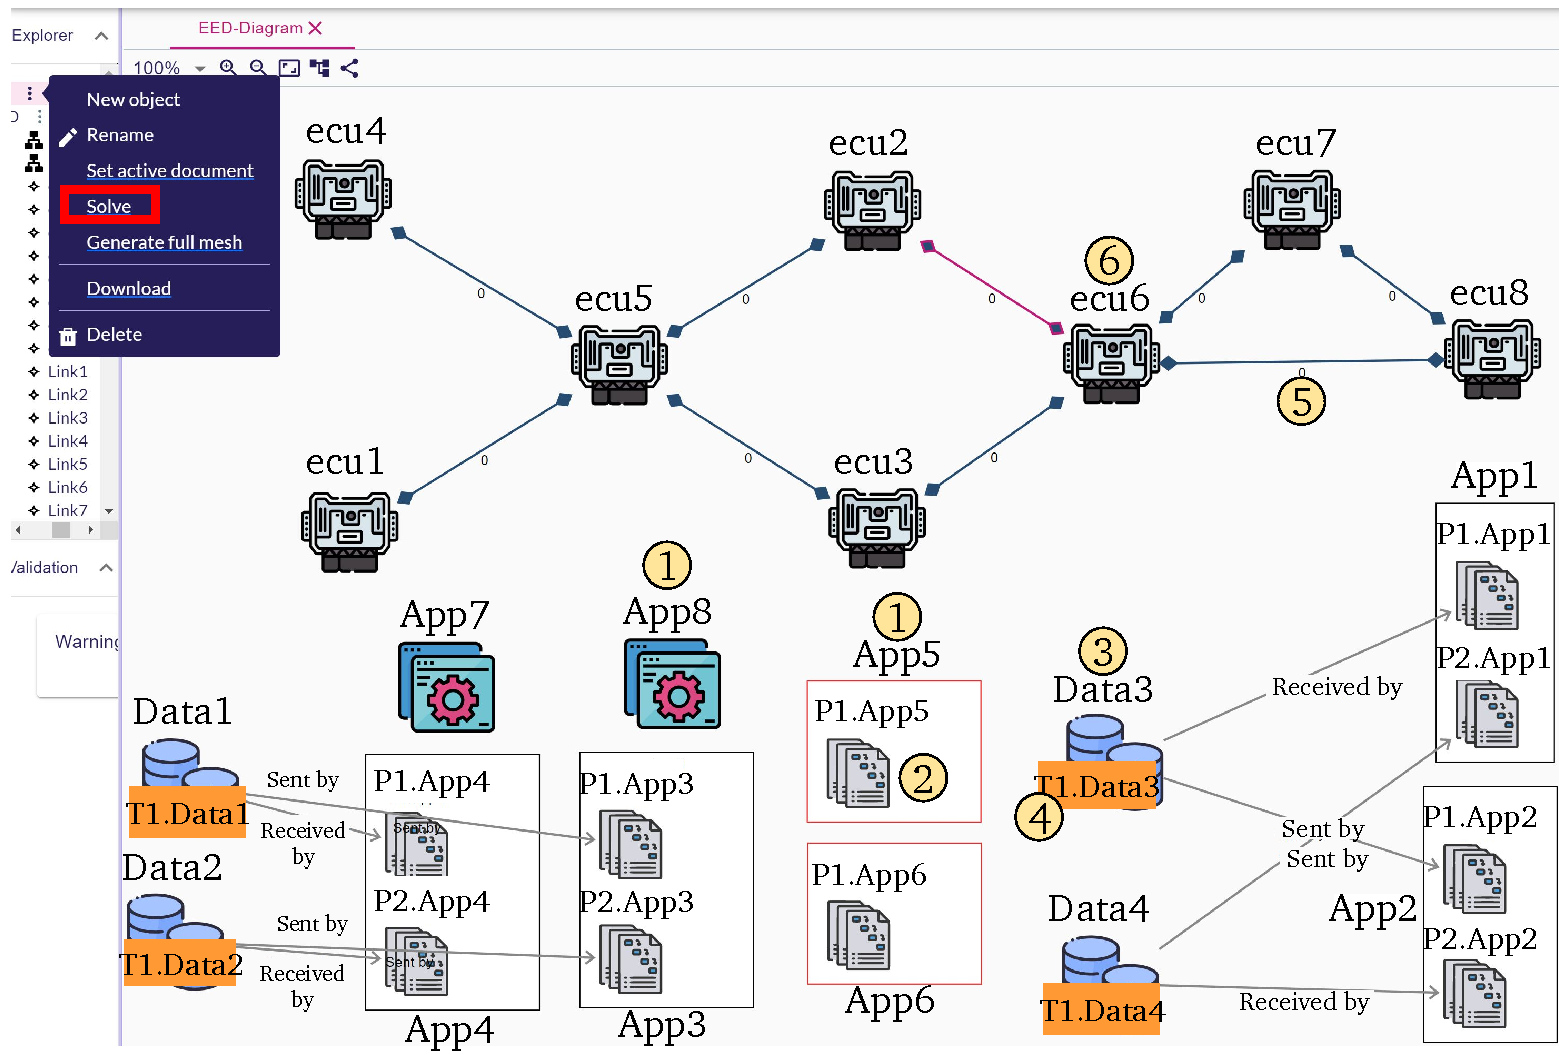
\includegraphics[width=1\textwidth]{figures/solved_model_new.pdf}
	\caption{A modeled E/E architecture by the presented tool including applications (No. one), application threads (No. two), communication messages (No. three), communication tasks (No. four), links (No. five), and ECUs (No. six). The model is solved and optimized by clicking on the \textit{Solve} option (red rectangle)~\cite{askaripoor2023designer}.}
	\label{fig7} 
    \end{figure}

    \subsection{Solving}
    
    To solve and optimize a created model considering the defined properties, requirements, and optimization objectives, e.g., the model shown in Figure~\ref{fig7}, a \textit{Solve} option is integrated~\cite{askaripoor2023designer}. Clicking on \textit{Solve} option enables the tool to solve the problems associated with the modeled architecture while optimizing the solution and satisfying the specified requirements, as described in Chapter~\ref{method}. In the model shown in Figure~\ref{fig7}, there are eight applications, six of which include one or two threads with the same periods and different execution times and two applications without a thread. Two applications here are selected as safety-critical (\textit{App$_{5}$} and \textit{App$_{6}$} shown with a red frame). Also, the model consists of four communication messages with the same periods as application threads and various frame lengths. It is aimed to automatically assign the applications to eight ECUs while meeting defined requirements. It is required to ensure that the threads running on each ECU have the correct time-triggered schedules and that all conditions for automated mapping of safety and non-safety-critical applications are fulfilled. 
    
    \begin{figure}[t]
 	\centering
 	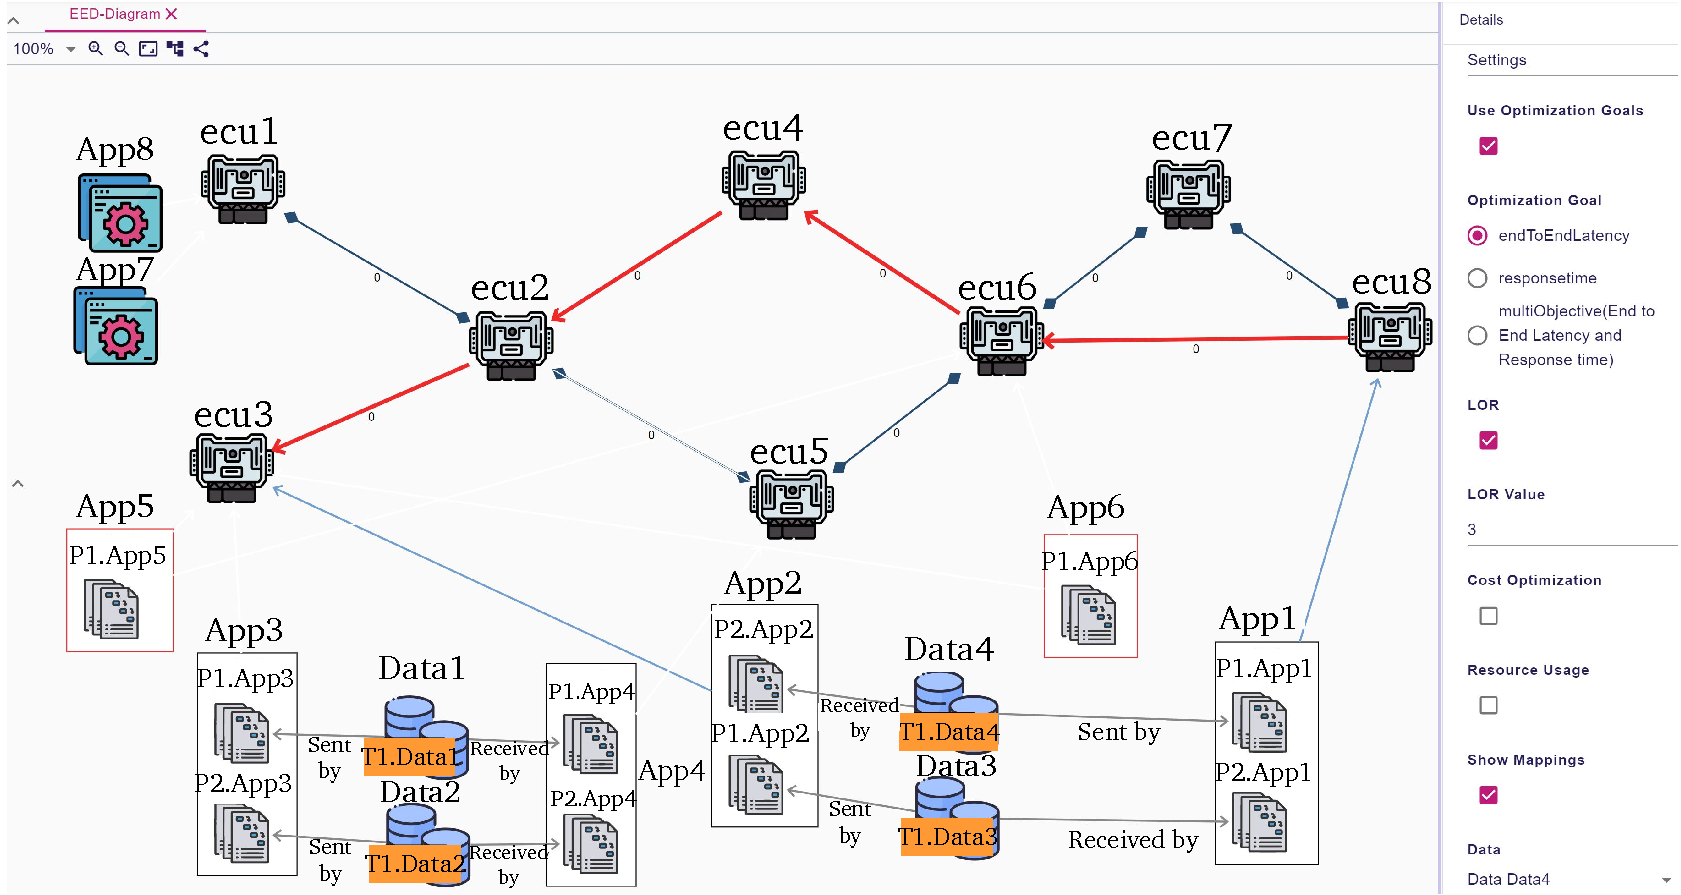
\includegraphics[width=1\columnwidth]{figures/ee_model_path.pdf}
 	\caption{A solution of the designed model in Figure~\ref{fig7} including mapping, message routing, and scheduling. Here, only the mappings for applications one and two related to the communication message four are displayed~\cite{askaripoor2023designer}.}
 	\label{fig8}
    \end{figure}
    
    %\begin{figure}[ht]
 	%\centering
 	%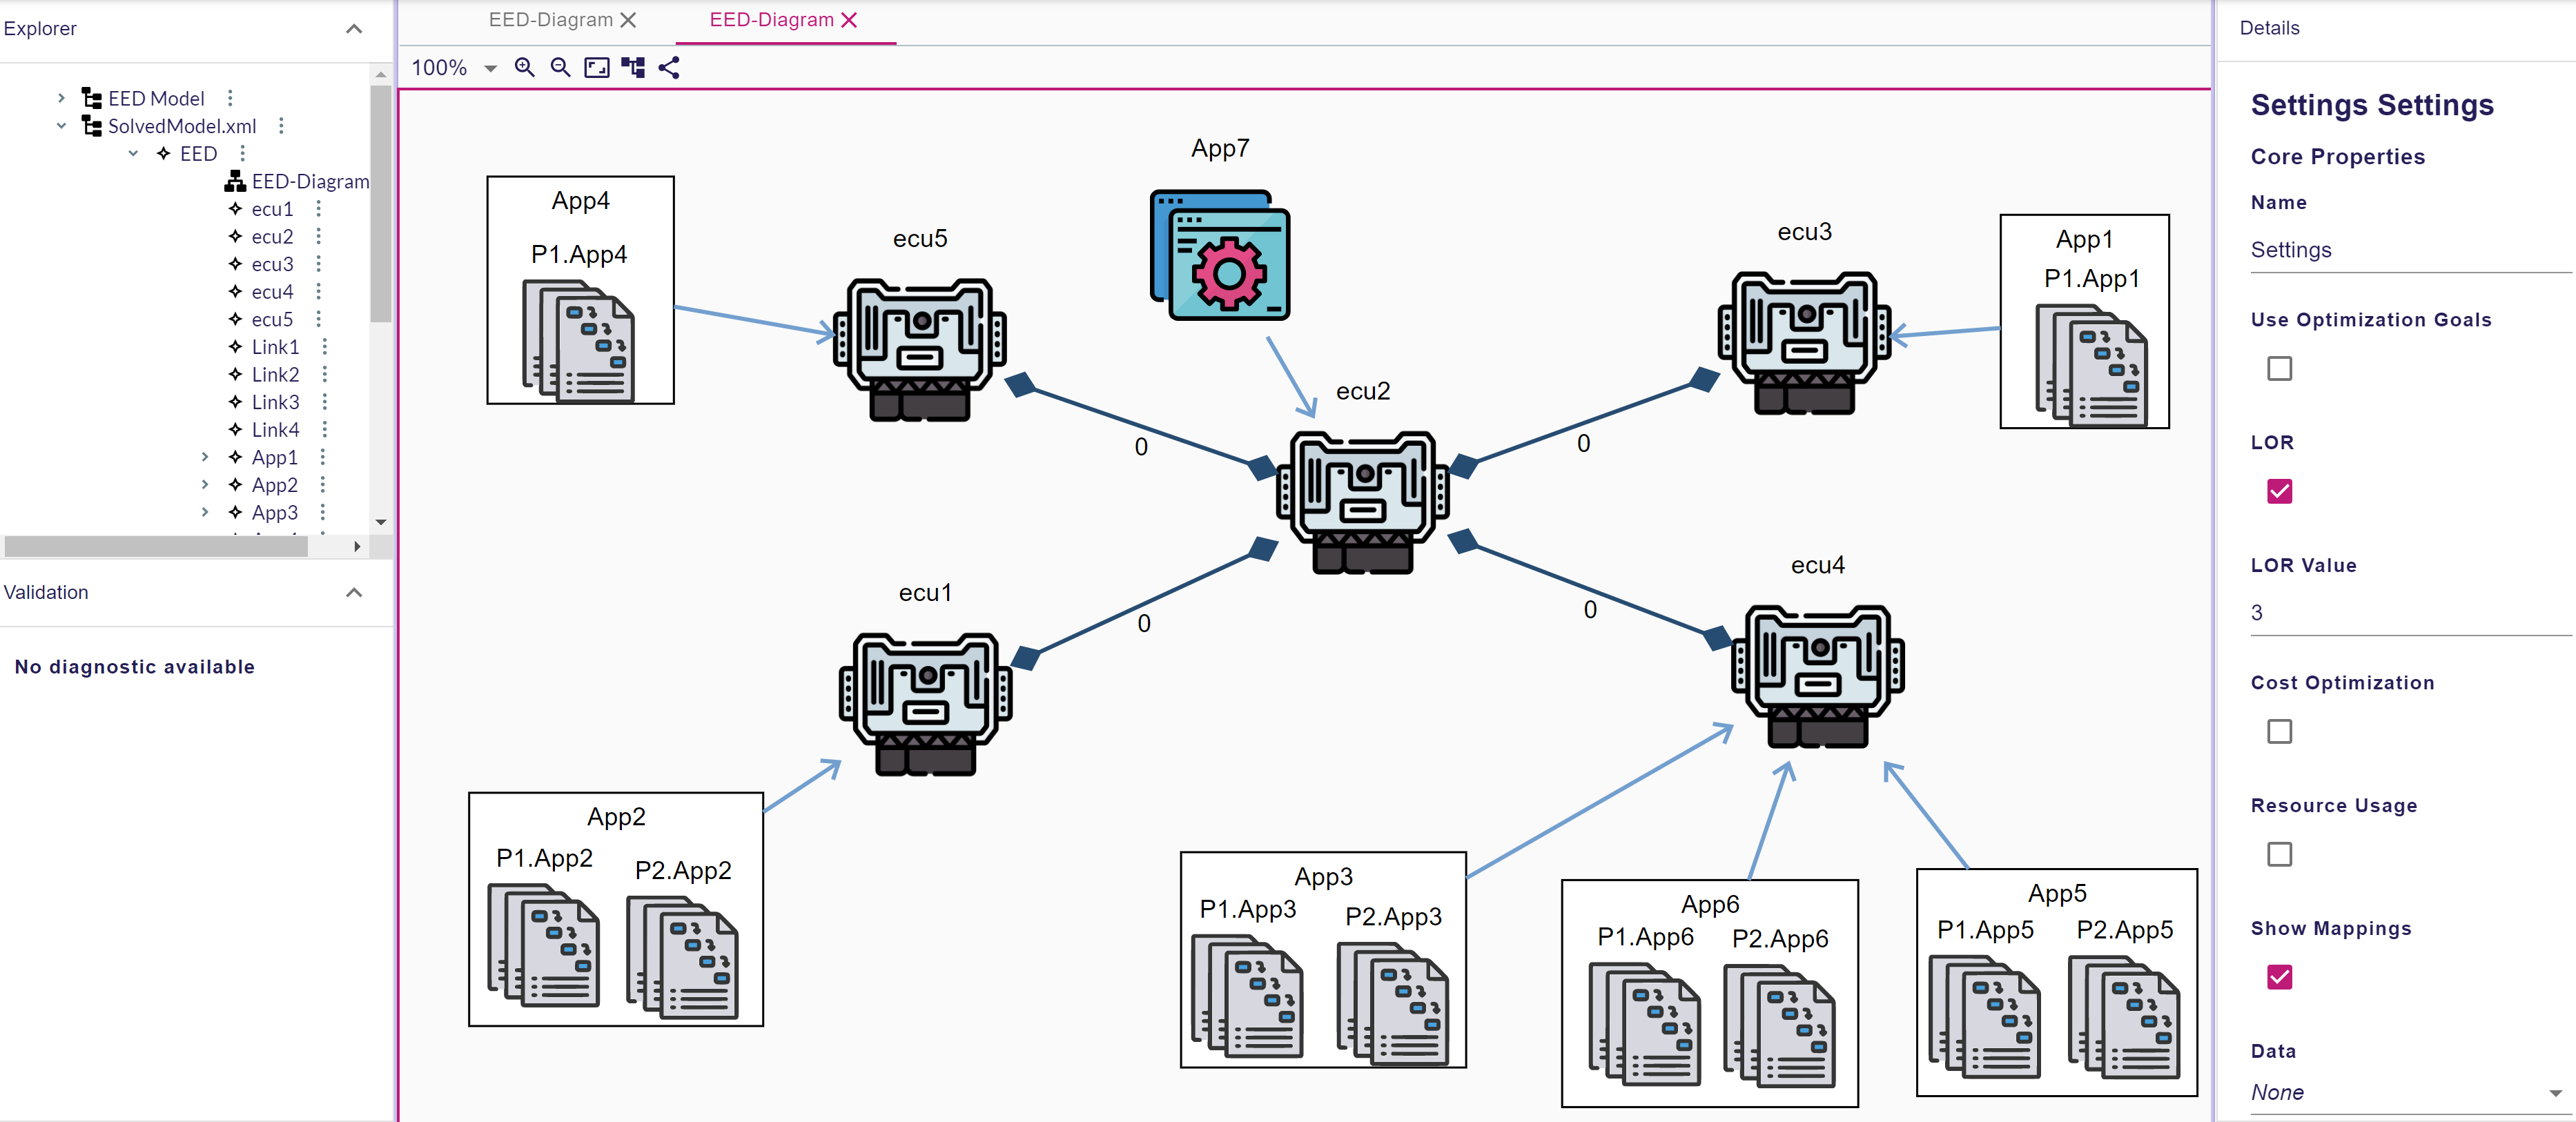
\includegraphics[width=1\columnwidth]{figures/solvedmapping1.PNG}
 	%\caption{The mapping solution of the presented model in figure~\ref{fig7}.}
 	%\label{fig8}
    %\end{figure}

    \subsection{Solutions}
     After getting the model solved, the user can observe the optimized solutions for mapping, scheduling of application threads and communications tasks, and message routing. Figure~\ref{fig8} displays the solution of the design model depicted in Figure~\ref{fig7}, which includes message routing, mapping, and scheduling for application threads and communication tasks~\cite{askaripoor2023designer}.

    
    \subsubsection{Mapping}
    
      %Therefore, as the mapping solution, figure~\ref{fig8} depicts which applications are assigned to which ECUs (blue arrows). As one of the defined requirements, each ECU must have at least one running application, encoded in constraint~(\ref{eq2}), which is met based on the solution. However, here only the mapped applications as a sender and a receiver related to a selected communication message are visualized. This applies due to avoiding confusion and cleanness of the model specially when the is model is extensive.
        
        
        
        %As the mapping solution is illustrated in figure\ref{fig8}, depicting the assignment of applications to specific ECUs through the representation of blue arrows. An essential condition dictates that each ECU must host a minimum of one operational application, a requirement formulated as a constraint in Chapter~\ref{method}. The presented solution effectively fulfills this requirement, ensuring its satisfaction.
        As a mapping solution, the E/E Designer tool determines which applications should be assigned to which ECUs (e.g., blue arrows in Figure~\ref{fig8}). The current mapping requirements in this example are redundancy conditions for safety-critical applications, and the constraint ensures that the threads running on each ECU are not the sender and receiver of the same communication message. In Figure~\ref{fig8}, only mappings related to sender and receiver applications of communication message $Data_4$ are visualized.
        
        It is important to note that the visualization in Figure~\ref{fig8} exclusively highlights the mapped applications functioning as both senders and receivers for a selected communication message (here, communication message number four). This design choice is motivated by enhancing clarity and comprehensibility within the model, mainly when dealing with extensive complexity. By focusing on this specific aspect, potential confusion is mitigated, resulting in a cleaner representation that facilitates a more intuitive understanding of the mapping scenario.
      
          \begin{figure}[ht]
    	\centering
    	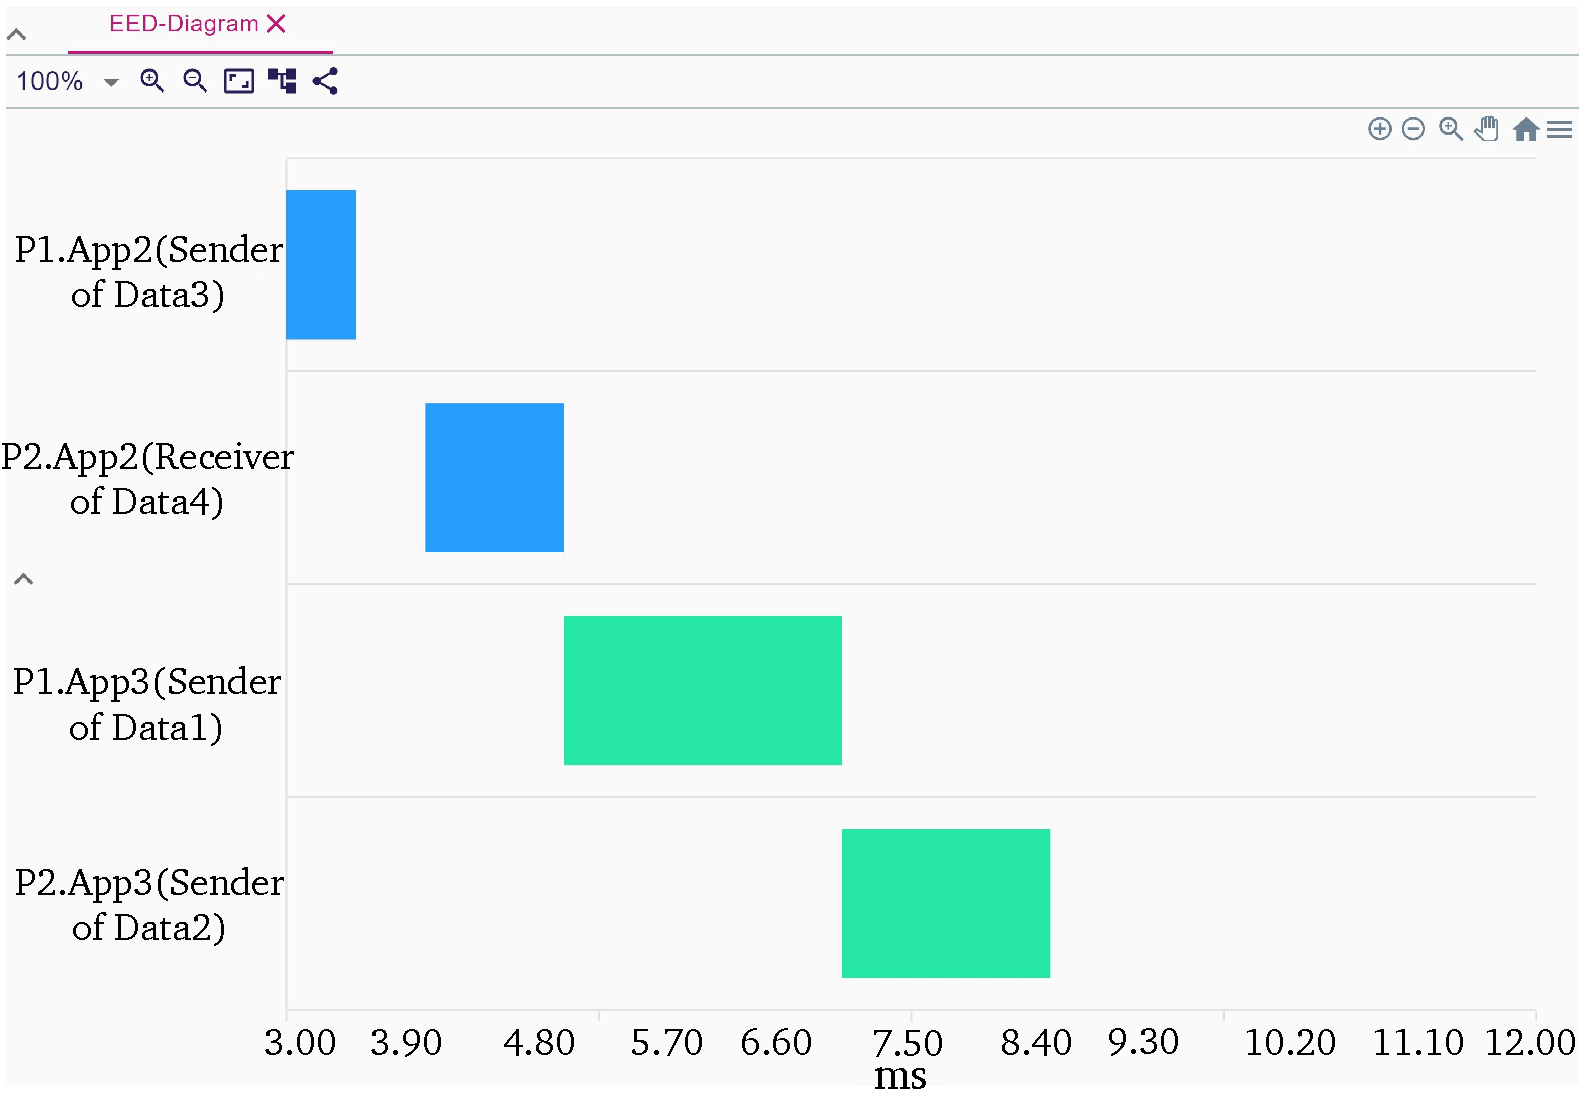
\includegraphics[width=0.85\columnwidth]{figures/schedule_new.pdf}
    	\caption{Calculated time-triggered schedules by the introduced tool for running application threads on~\textit{ECU$_3$} after mapping action as the solution for the model in Figure~\ref{fig8}~\cite{askaripoor2023designer}.}
    	\label{fig9}
        \end{figure}  
    \subsubsection{Time-triggered Scheduling for Application Threads}
    
         Figure~\ref{fig9} shows the calculated schedules for the application threads executing on \textit{ECU$_3$} in Figure~\ref{fig8} within a computed hyperperiod. As can be observed, each color represents an application, and each slot indicates a thread's schedule. Each slot may be executed multiple times within the hyperperiod, depending on the thread's period. Figure~\ref{fig0009} presents another example of a mapping schedule related to 20 threads executing on an ECU.  
    
    
    
    %Moreover, figure~\ref{fig9} shows the calculated schedules for the application threads executing on~\textit{ECU$_4$} in a computed hyperperiod. As can be observed, each color represents an application, and each slot indicates a thread's schedule. Depending on the thread's period, it can be executed multiple times in the hyperperiod. For example, the last row shown in figure~\ref{fig9}, \textit{P$_2$.App$_3$}, which is one of the threads of \textit{App$_3$}, is executed once in the hyperperiod.
       
       
       
      
        
        \begin{figure}[b!]
    	\centering
    	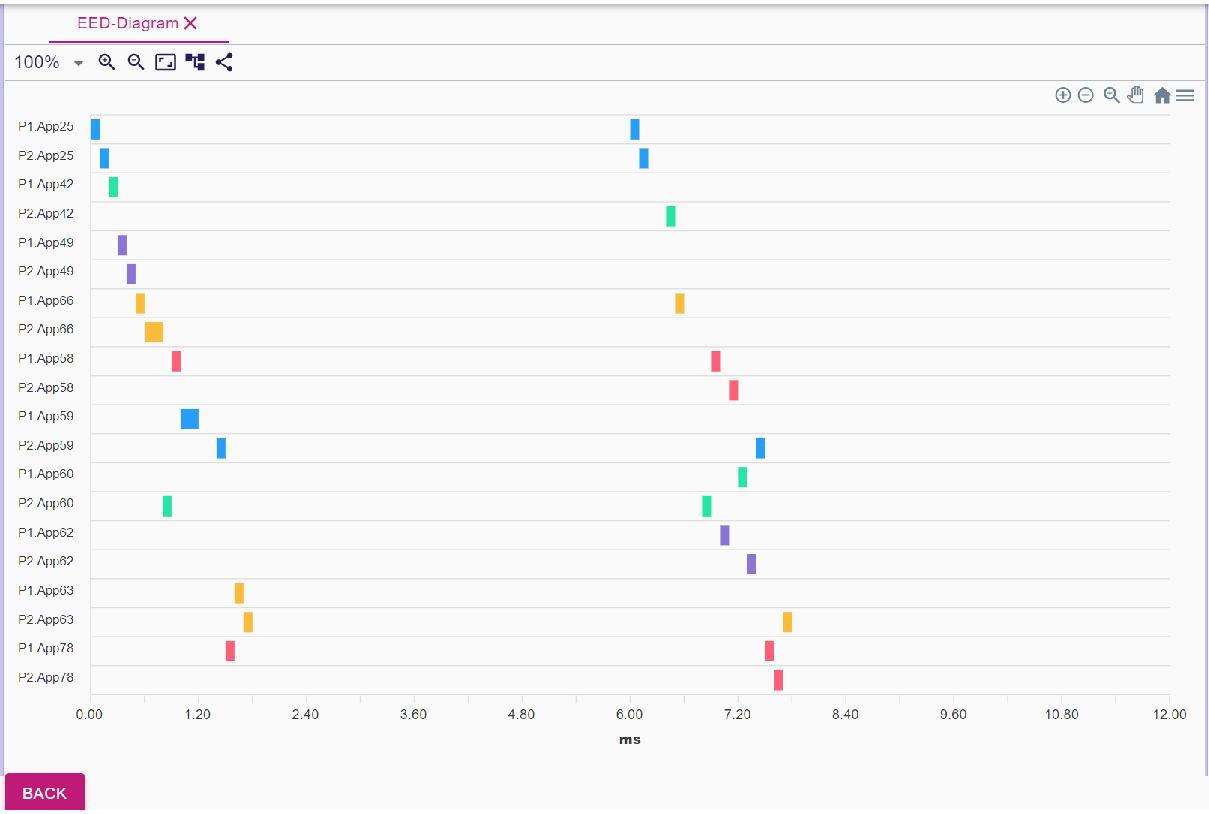
\includegraphics[width=0.9\columnwidth]{figures/20processes_schedule.pdf}
    	\caption{Computed time-triggered schedules by the introduced tool for running 20 application threads belonging to 10 applications on an ECU after mapping action.}
    	\label{fig0009}
        \end{figure}
        
                \begin{figure}[ht]
	    \centering
	    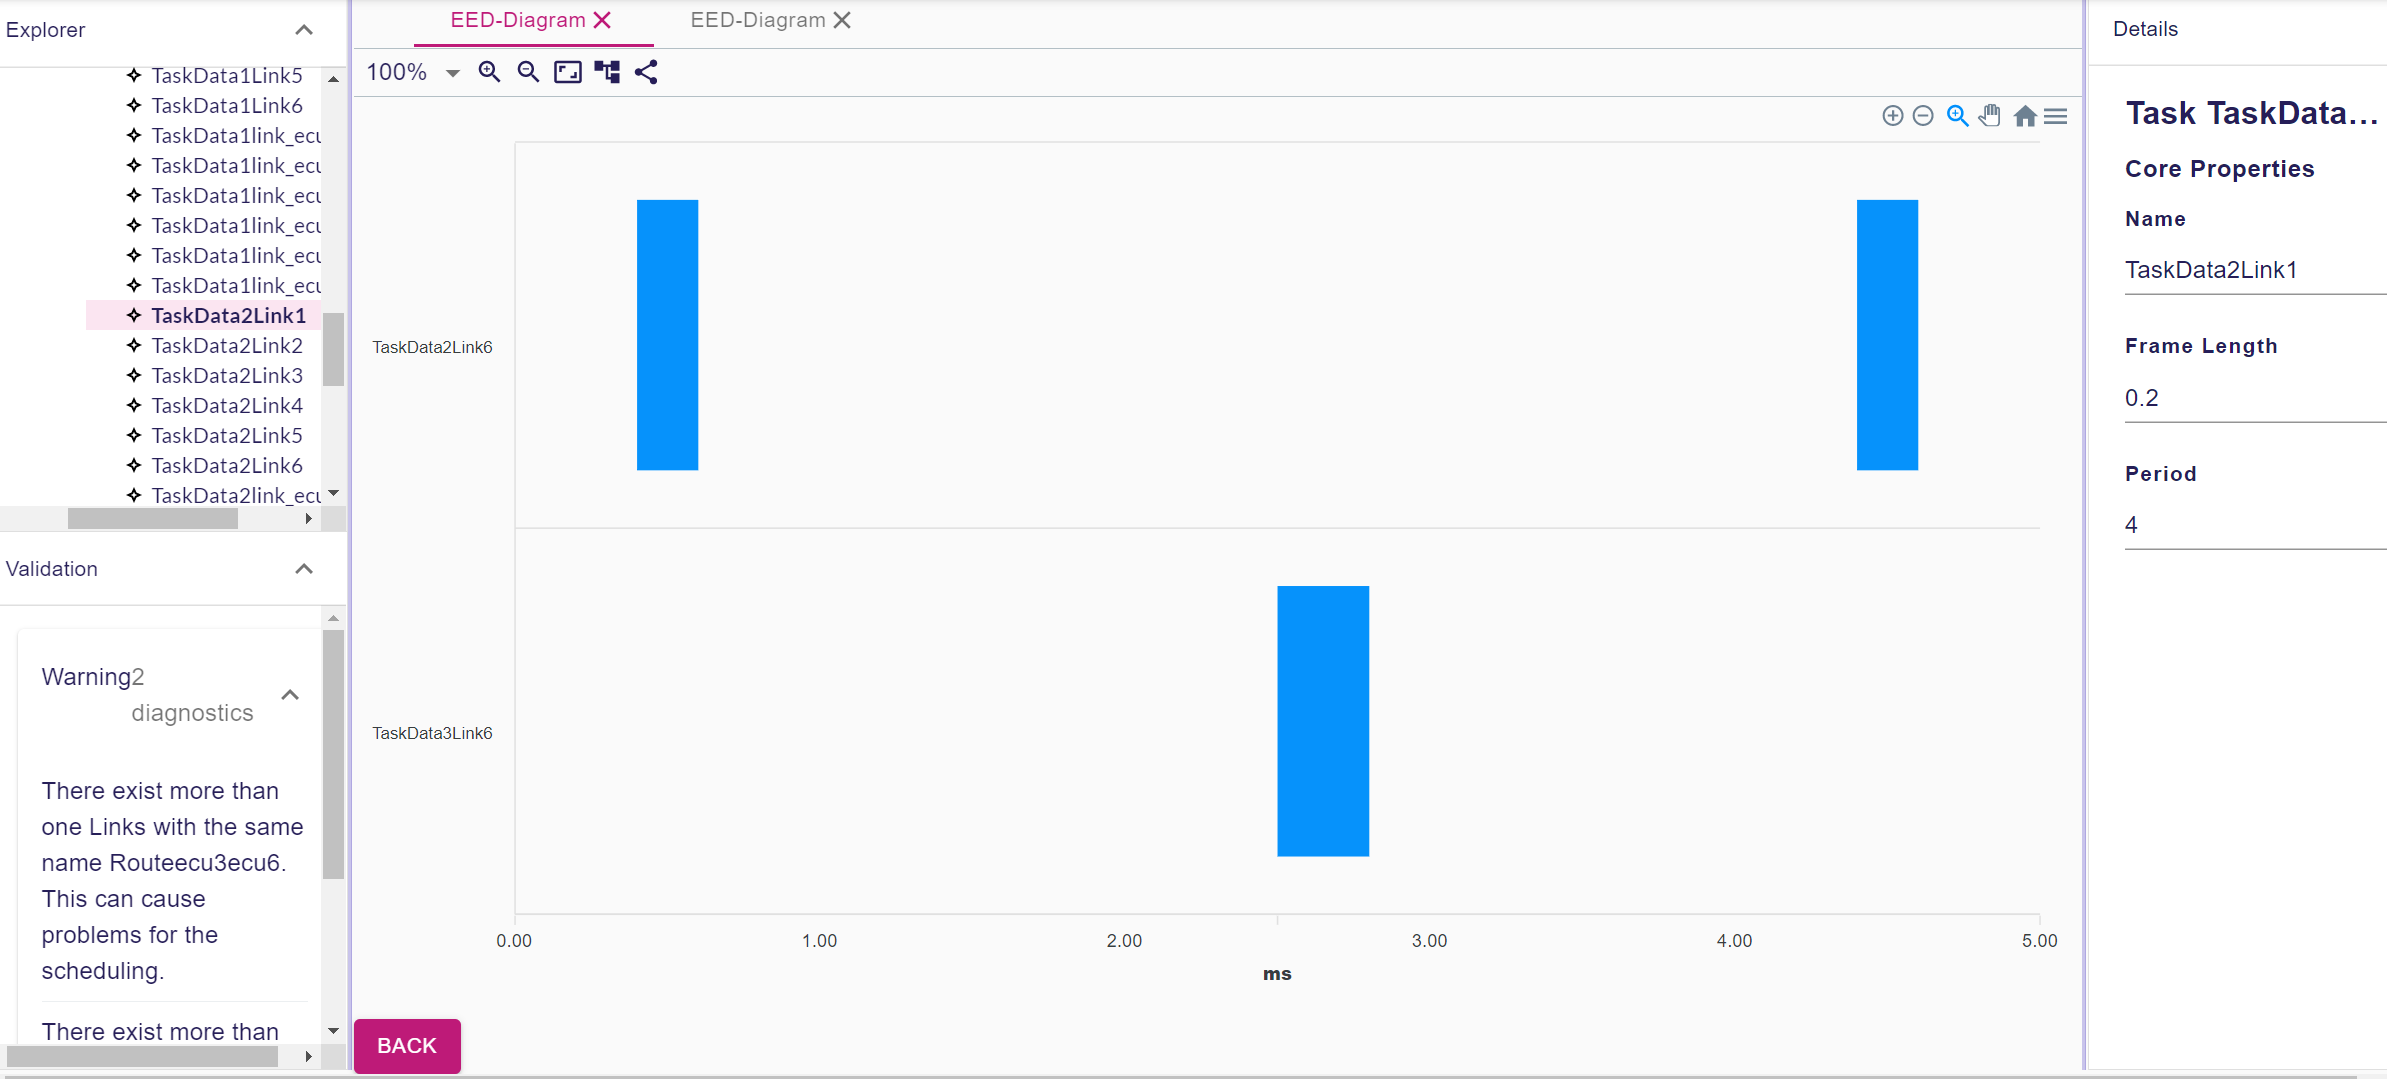
\includegraphics[width=0.9\columnwidth]{figures/schedule_link.PNG}
	    \caption{Time-triggered schedules of two communication tasks over a link.}
	    \label{fig11}
        \end{figure}
        \subsubsection{Communication Message Routing}
       % A created route for a specific communication message to route the message from a sender to a receiver can be shown in the frontend. As an example, figure~\ref{fig10} displays a solution of a designed model beforehand, including the message routing, mapping, and scheduling for threads and communication tasks. We skip the mapping part and its scheduling since they were explained in the previous model. In Fig.~\ref{fig10}, there are three communication messages which need to be sent from senders to receivers. As explained before, each message comprises a communication task routing over the network links, and the user must select the threads as the sender and receiver of each message in the front end before the solving step. Therefore, after solving the model, the user can observe the correct path for each communication message by choosing a desired message.
  
        A created route for a specific communication message to route a message from a sender to a receiver can be shown in the frontend. In Figure~\ref{fig8}, four communication messages need to be sent from senders to receivers. As described in Chapter~\ref{method}, each message comprises a communication task routing over the network links, and the user must specify the threads as the sender and receiver of each message in the frontend before the solving step. Therefore, after solving the model, the user can observe the correct path for each communication message and related mappings for sender and the receiver applications relevant to the same communication message by choosing a desired message. Based on Figure~\ref{fig8}, the red path shows a generated route from \textit{ECU}$_8$ as a sender to a receiver \textit{ECU}$_3$ routing the communication message~$d_4$.
        
        
        
        \subsubsection{Time-triggered Scheduling for Communication Tasks}
        
        Similar to the scheduling for application threads, the communication task slots are displayed during the related hyperperiod. It should be added that end-to-end latency optimization goal was applied in the solution presented in Figure~\ref{fig8}. In addition, the computed time-triggered schedules for four communication tasks routed over links can be visualized similarly to Figures~\ref{fig9} and \ref{fig0009}. For example, Figure~\ref{fig11} illustrates correct schedules for two communication tasks over a link. Also, in Figure~\ref{fig11}, each row relates to each communication task relevant to a specific message.
        
        
        \begin{comment}
        \begin{figure}[ht]
    	\centering
    	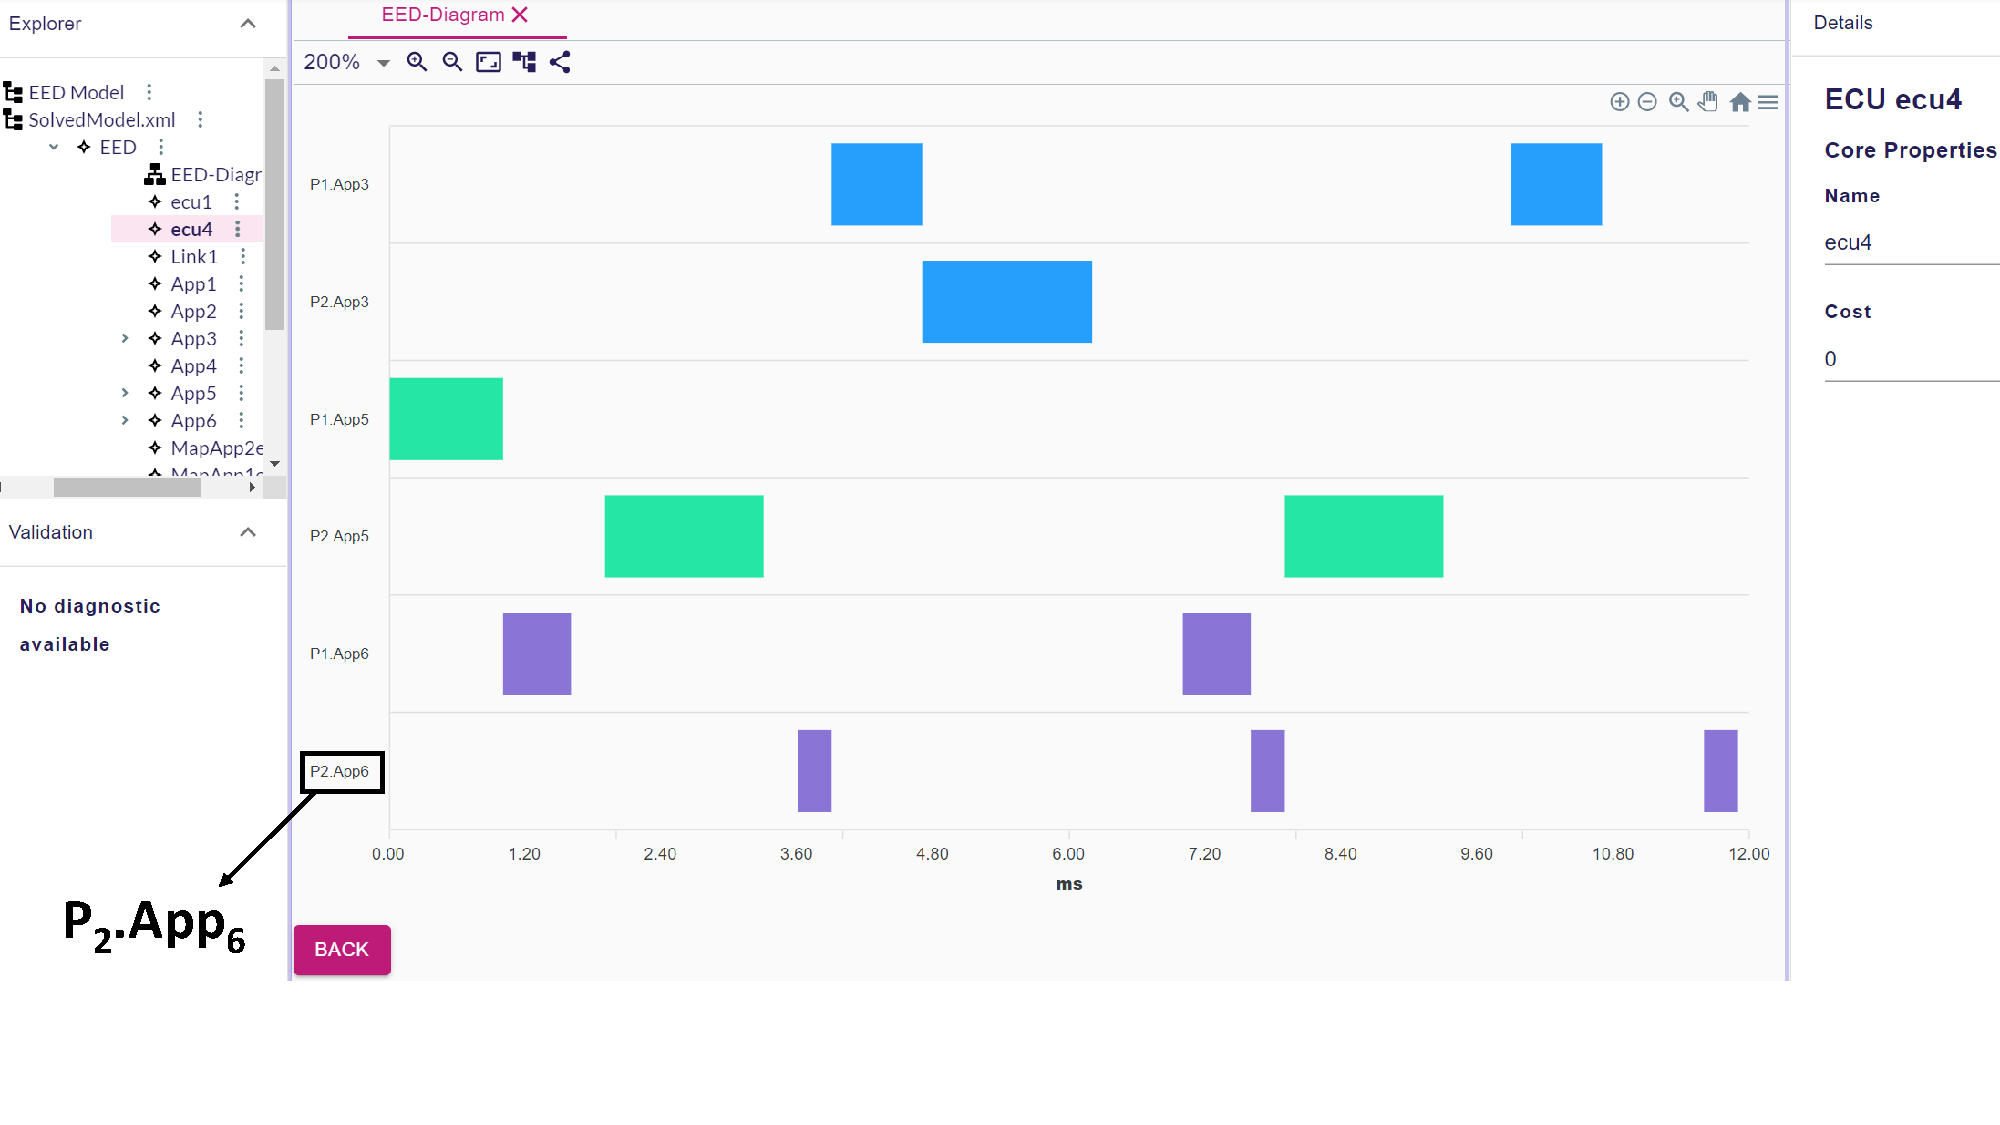
\includegraphics[width=1\columnwidth]{figures/scheduling_ecu4_n2.pdf}
    	\caption{Visualization of calculated schedules for running threads on~\textit{ECU$_4$} in the mapping solution displayed in figure~\ref{fig8}.}
    	\label{fig9}
        \end{figure}
        \end{comment}
    
    

    
    %Based on the Fig.~\ref{fig10}, the red path shows a generated route from \textit{ECU}$_1$ as a sender to a receiver \textit{ECU}$_6$ routing the communication message~$D_1$ after selecting by the user. In addition, the computed time-triggered schedules for two communication tasks routed over a link are visualized in Fig.~\ref{fig11}.

    %Similar to the mapping, the task slots are displayed during the related hyperperiod. It should be added that no optimization objectives have been applied in this solution.
    \section{Model Validation}
    
    Model validation plays a crucial role in ensuring the accuracy, reliability, and quality of an E/E model created using a modeling tool. %E/E architecture modeling tools enable engineers to represent the complex interconnections, components, and functionalities of E/E systems in a visual and systematic manner. 
     To effectively utilize the tools for architectural design, it is essential to validate the models against various criteria and requirements.
    Model validation involves systematically examining and verifying the E/E architecture model to ensure that it conforms to the desired specifications, standards, and constraints. It aims to identify and rectify potential errors, inconsistencies, or design flaws that can impact the final system's performance, safety, or reliability.
    When modeling an E/E system, validation encompasses multiple aspects. First, it involves verifying the correctness and coherence of the model's structure and behavior. This includes ensuring that the components, interfaces, signals, and their interactions are accurately represented. Moreover, the validation checks the model's compliance with domain-specific guidelines and defined requirements.
    Furthermore, model validation focuses on assessing the consistency and completeness of the model. It involves analyzing whether the model adequately captures all the necessary system requirements, functional specifications, and performance constraints. System integrators can detect missing or ambiguous requirements, redundant or conflicting specifications, and incomplete or inaccurate representations by conducting thorough validation.    
    Another critical aspect of model validation in E/E architecture modeling tools is the evaluation of system properties and performance attributes. For example, in the case of safety requirements, if the user assigns an ASIL D application to a core of an HPCU which does not support ASIL D, the validation process gives a warning to the user. Hence, the validation process ensures that the model adheres to these properties and meets the necessary performance targets.
            \begin{figure}[t]
    	\centering
    	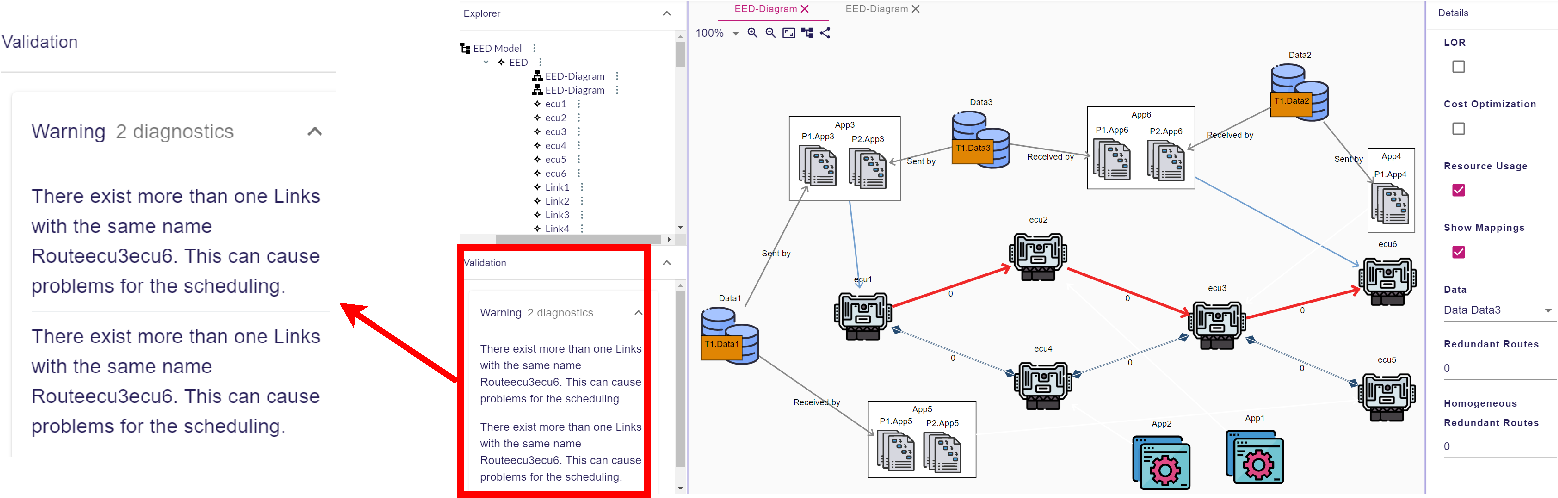
\includegraphics[width=1\columnwidth]{figures/validation.pdf}
    	\caption{A solution of a modeled E/E topology including mapping and message routing. On the left side, several warnings are displayed regarding the validation of the model.}
    	\label{fig10}
    \end{figure}
    %Model validation also involves validating the model against real-world scenarios and use cases. This can be achieved through simulations, tests, or formal verification techniques. By subjecting the model to various scenarios, engineers can assess its behavior, identify potential issues, and evaluate the system's performance under different operating conditions.
    
    %%Effective model validation requires a combination of manual inspection, automated checks, and rigorous testing methodologies. It is an iterative process that should be performed at different stages of the modeling lifecycle, from initial design to system integration. Additionally, as the E/E architecture evolves or new requirements emerge, the model should be continuously validated and updated to ensure its accuracy and relevance.
    
    Since several different model requirements must be met to create a valid model, as explained above, errors, warnings, and general tips can assist the user in having a valid model. The validation of the introduced tool is a continuous process, checking the model after each change and displaying validation messages if required. The message validation consists of a problem description and includes the elements, mappings, or attributes that lead to an issue. Moreover, the message indicates the acuteness of the problem and the urgency to change the model~\cite{askaripoor2023designer}. Based on
    this, three different message types are introduced, including \textit{error}, \textit{warning}, and \textit{message} that each of them are described in the following. 

    \subsubsection{Error}
      %An \textit{error} appears if a model violation occurs. That breaks critical safety requirements or leads to MIP constraints violation. This message type implies that the user must change the model in order to fix the error.
      
    An \textit{error} occurs when there is a violation in the model, which disrupts critical safety measures or breaks the rules of MIP constraints~\cite{askaripoor2023designer}. This message indicates that the user needs to adjust the model to fix the error. Promptly addressing such errors is crucial, as they not only affect how well the system works but also endanger the overall reliability of the system.
      
    \subsubsection{Warning}
    A \textit{warning} serves as an advisory signal intended to highlight potential violations or discrepancies that, while not necessarily leading to critical problems, merit attention and rectification~\cite{askaripoor2023designer}. It points out areas of concern that should be addressed to enhance the overall quality and effectiveness of the subject under consideration. For instance, as illustrated in Figure \ref{fig10}, the designed model is accompanied by a series of \textit{warnings}. These cautionary indications shed light on aspects of the model's design that may not align with best practices or desired standards. While these warnings may not immediately result in severe issues, they serve as essential signposts that prompt further investigation and possible adjustment. Ignoring such warnings can lead to compounded issues or hinder the model's optimal performance.


    
    %While, a \textit{warning} is used for violations that should not be done but do not cause a severe issue. For instance, in Fig.\ref{fig10}, there are several \textit{warnings} for the designed model.
    
    \subsubsection{Message}
    %Finally, the system shows a \textit{message} for simple tips, notes, and other information.
    
    Finally, the system displays a \textit{message} to provide users with helpful tips, essential notes, and additional information. This feature aims to enhance the user experience by offering valuable insights and guidance~\cite{askaripoor2023designer}. Whether it is a brief pointer to optimize their workflow or a noteworthy caution about potential pitfalls, these messages serve as a valuable resource to users, aiding them in making informed decisions and using the system more effectively.
    
    
    
   




\section{Implementation}
    
    This section discusses the prototypical implementation of the E/E Designer's frontend.
    As Chapter~\ref{method} mentioned, the Eclipse IDE platform was selected as the development environment. The Eclipse IDE supports various plugins for Java that assist in the development process. One of the main plugins used in this project was the eclipse modeling framework (EMF), which Sirius and Sirius Web utilize for creating class models and aiding in code generation~\cite{eclipse}.
    
           \begin{figure}[b!]
    	\centering
    	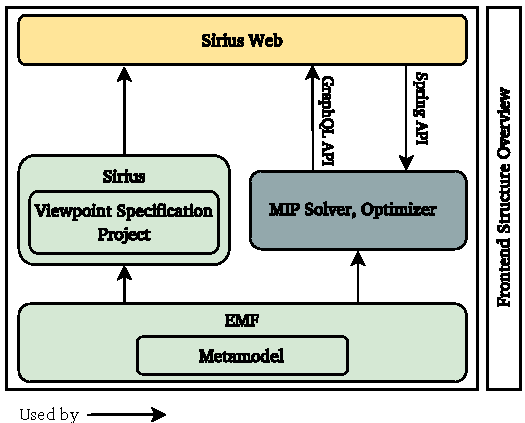
\includegraphics[width=0.7\columnwidth]{figures/frontend_st1.pdf}
    	\caption{An outline of the proposed framework's frontend describing the interaction of modified \textit{Sirius Web} with other modules existing in the backend.}
    	\label{fig12}
    \end{figure}
    
    \subsection{Sirius Web}
     
     \textit{Sirius Web} is used as the front-end's foundation of the E/E Designer to provide the web-based functionality. It is an open-source web-based extension of \textit{Sirius Desktop}. Eclipse \textit{Sirius Web} is a framework to easily create and deploy studios to the web~\cite{siriusweb}.
     By using the \textit{Sirius Web}, the modeling features of \textit{Sirius} can directly be utilized from a web browser. Once the \textit{Sirius Web} is deployed on a server, %it can be run from a web browser without specific installation on the user's desktop, so that it allows users to simultaneously access and modify editing contexts, and also download and upload projects
     users can access and modify editing contexts and download and upload projects without requiring specific installation on their desktops~\cite{siriusweb}.
     To integrate all defined attributes, functional requirements, boundary constraints, and optimization objectives specified in the E/E Designer backend as explained in the Chapter~\ref{method}, the \textit{Sirius Web} has been modified and developed to provide an appropriate frontend for the introduced tool. Furthermore, all outputs generated by the framework, such as mapping, routing, and scheduling, can be visualized by the developed frontend. The Figures \ref{fig5} to \ref{fig10} shown above are screenshots from the E/E Designer frontend, which is based on the \textit{Sirius Web}.\newline 
     
    %figure~\ref{fig12} depicts an overview of how the frontend (i.e., modified \textit{Sirius Web}) interacts with other modules integrated in the backend. The EMF plugin provides the possibility to create a metamodel which then can be used byother plugins. The metamodel is utilized by the MIP solver and optimizer (the E/E Designer uses the Gurobi Solver as mentioned in the Chapter~\ref{method}) and by \textit{Sirius}. The \textit{Sirius} is the local version of the \textit{Sirius Web} and it is technically is a sub-project of the \textit{Sirius}. The \textit{Sirius} knows through the model which object classes exist and how they are related to each other. This enables the \textit{Sirius} to define howeach instance object should look like and behave.The \textit{Sirius Web} reuses some functionality of Sirius. %In this case the odesign file from Sirius which specifies the rules and designs used for the model must be integrated into Sirius Web.There is also the distinction of the system between the frontend part which is usingJavaScript and the backend part which uses Java. Both systems must interact with each other.As two separate programming languages cannot directly communicate with each other an interface is needed. Therefore, the \textit{Sirius Web} comes natively with a GraphQL interface whichcan provide different kinds of data and offers methods for uploading data. For the Java component the Spring Framework is used. Within the development process, a call to a Spring method is executed once an user wantsa model solved or requests other features e.g., full-mesh generation. After the solver solves the model, the GraphQLAPI is utilized to upload a new model to the \textit{Sirius Web} where it is available for the user in theweb-interface.
    
    Figure~\ref{fig12} presents an overview of how the frontend (i.e., modified \textit{Sirius Web}) interacts with other modules integrated in the backend. The EMF plugin allows creating a metamodel, which other plugins can then utilize. The metamodel is employed by the MIP solver and optimizer (the presented tool uses the Gurobi Solver as mentioned in Chapter~\ref{method}) and by \textit{Sirius}. \textit{Sirius} is the local version of \textit{Sirius Web} and is technically a sub-project of \textit{Sirius}. \textit{Sirius} identifies the existing object classes and their relationships through the model. This enables \textit{Sirius} to define the appearance and behavior of each instance object.
    \textit{Sirius Web} reuses some of the functionality of Sirius. A distinction is also made within the system between the frontend, which uses JavaScript, and the backend, which employs Java. Both systems need to interact with each other. An interface is required since two separate programming languages cannot directly communicate. Therefore, \textit{Sirius Web} comes natively with a GraphQL interface that offers various types of data and methods for data uploading. For the Java component, the Spring Framework is used. A call to a Spring method is executed in the development process when a user wants a model solved or requests other features, such as full-mesh generation. After the solver completes solving the model, the GraphQL API uploads the new model to \textit{Sirius Web}, where it becomes available for the user in the web interface.
    %\null
    %\addtocounter{page}{1}
    %\newpage
    %\thispagestyle{empty}
